\documentclass[pdf, aspectratio=169, 12pt]{beamer}
\usepackage[]{hyperref, graphicx, siunitx, lmodern, tikz, booktabs, physics, multicol}
\usepackage[mode=buildnew]{standalone}
\usepackage{pdfpc-commands}
\usepackage{pgfplots}
\pgfplotsset{compat=1.16}

\usetheme{Python}

\graphicspath{ {Images/} }

\sisetup{per-mode=symbol}
\usetikzlibrary{calc, patterns, decorations.markings, decorations.pathmorphing, shapes, fit}

%Preamble
\title{Plotting some classy arcades}
\author{Jed Rembold}
\date{April 13, 2020}

\begin{document}

\begin{frame}{Announcements}
	\begin{itemize}
		\item Homework
			\begin{itemize}
				\item Homework 10 posted!
				\item Should already be able to do Problem 1 after today, and Problem 2 by Wednesday
			\end{itemize}
		\item My quest to get caught up on grading continues, expect at least mostly up-to-date grade reports soon
		\item Information on semester-ending project coming end of the week
		\item Polling: \nolinkurl{rembold-class.ddns.net}
	\end{itemize}
\end{frame}

\begin{frame}[fragile]{Review Question}
	\vspace{-5mm}
	\begin{columns}
		\column{0.4\textwidth}
		\column{0.6\textwidth}
		{\small
			\begin{pythoncode}
				import matplotlib.pyplot as plt
				f = plt.figure()
				axa = f.add_subplot(122)
				axb = f.add_subplot(121)
				axa.plot([5,4,3,2,1], 'ro-')
				plt.show()
			\end{pythoncode}
		}
		
	\end{columns}
	
	Which plot below would result from the above code?
		\vspace{5mm}
		\hspace*{-5mm}
			\begin{tikzpicture}
				\node[label={above:A}](A) at (0,0) {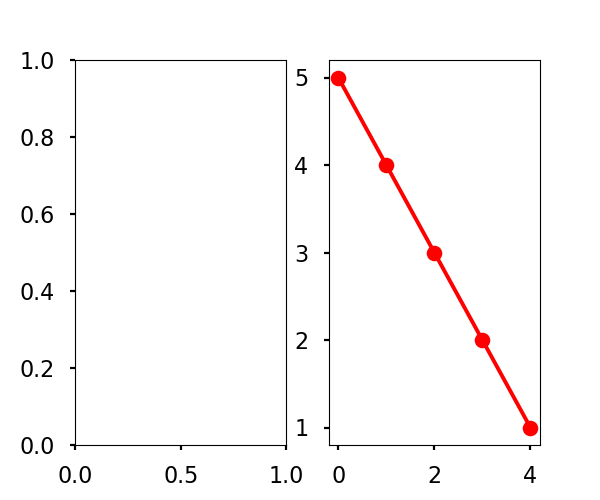
\includegraphics[width=3.5cm]{Code/SolA.png}};
				\node[right = 1pt of A, label={above:B}](B) {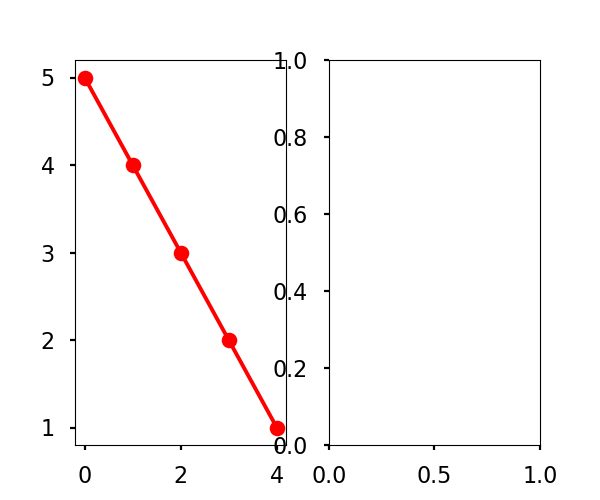
\includegraphics[width=3.5cm]{Code/SolB.png}};
				\node[right = 1pt of B, label={above:C}](C){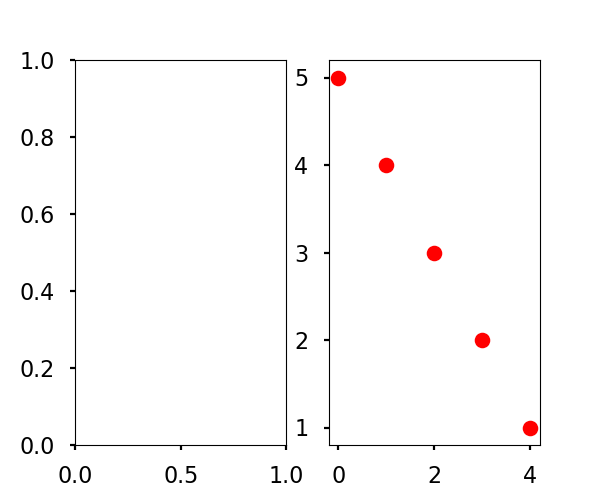
\includegraphics[width=3.5cm]{Code/SolC.png}};
				\node[right = 1pt of C, label={above:D}](D){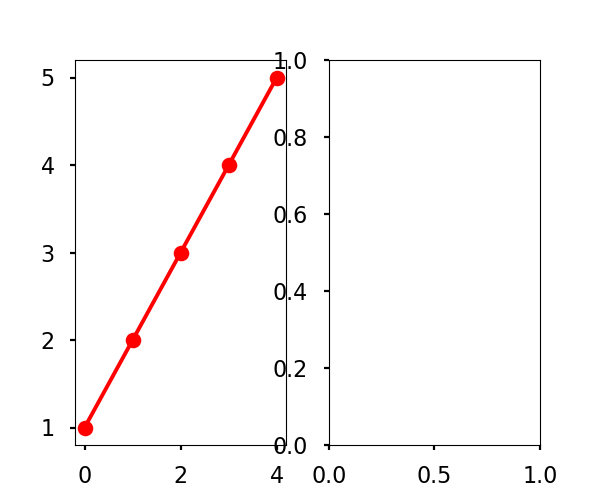
\includegraphics[width=3.5cm]{Code/SolD.png}};
			\end{tikzpicture}
\end{frame}


\begin{frame}{Extra Figure and Axes Features}
	\begin{itemize}
		\item Clear communication is important with visualization
		\item<+-> Should always include meaningful and descriptive axes label and figure titles.%
			\begin{itemize}
				\item Axes labels controlled with \pyi{.set_xlabel()} and \pyi{.set_ylabel()}
				\item Axes title controlled with \pyi{.set_title}
				\item Figure title controlled with \pyi{.suptitle}
			\end{itemize}
		\item<+-> Adjust tick spacing or labels:
			\begin{itemize}
				\item Customize autoscale limits: \pyi{.set_xlim()} or \pyi{.set_ylim()}
				\item Exactly where ticks appear: \pyi{.set_xticks()} or \pyi{.set_yticks()}
				\item What labels they have: \pyi{.set_xticklabels()} or \pyi{.set_yticklabels()}
			\end{itemize}
		\item<+-> Overall plot style:
			\begin{itemize}
				\item See available styles with \pyi{plt.style.available}
				\item Use with \pyi{plt.style.use('name of style')}
			\end{itemize}
	\end{itemize}
\end{frame}

\begin{frame}{Shared Axes}
	\begin{itemize}
		\item Commonly might want to shared an axis in a plot
			\begin{itemize}
				\item Overlaying plots on overlapping axes
				\item Side by side plots with linked axes
			\end{itemize}
		\item Easy method for overlapping:
			\begin{itemize}
				\item Use \pyi{.twinx()} or \pyi{.twiny()}
				\item Will automatically add the new axis to the opposite side of the plot as the current axis
			\end{itemize}
		\item For more manual control:
			\begin{itemize}
				\item Use \pyi{sharex} and \pyi{sharey} options when creating the axes object
			\end{itemize}
	\end{itemize}
\end{frame}

\begin{frame}{Types of Plots}
	\begin{columns}
		\column{0.5\textwidth}
		\begin{itemize}
			\item Heatmaps: \pyi{.imshow()}
			\item Contours: \pyi{.contour()}
			\item Histograms: \pyi{.hist()}
			\item Bar plots: \pyi{.bar()} or \pyi{.barh()}
			\item Pie Charts: \pyi{.pie()}
		\end{itemize}
		\column{0.5\textwidth}
		\begin{center}
			\includegraphics<1>[width=0.8\textwidth]{Heatmap.png}
			\includegraphics<2>[width=0.8\textwidth]{Contour.png}
			\includegraphics<3>[width=0.8\textwidth]{Histogram.png}
			\includegraphics<4>[width=0.8\textwidth]{BarPlot.png}
			\includegraphics<5>[width=0.8\textwidth]{PieChart.png}
		\end{center}
		
	\end{columns}
\end{frame}

%\begin{frame}{Intro to Graphics}
	%\begin{itemize}
		%\item Sometimes need more than just graphical output
			%\begin{itemize}
				%\item Or need smoother interface for real-time graphics
			%\end{itemize}
		%\item Python's standard graphical user interface tool is Tkinter
			%\begin{itemize}
				%\item Can be cumbersome to use when learning
			%\end{itemize}
			%\item We will use the more streamlined \pyi{graphics.py}
				%\begin{itemize}
					%\item A library build on top of Tkinter to make it easier to use
					%\item Make sure you grab the provided file and put it in the same directory as your script!
				%\end{itemize}
	%\end{itemize}
%\end{frame}

\begin{frame}{A Classy Arcade}
	\begin{itemize}
		\item We've been using \pyi{arcade} throughout the semester, but not to its full potential
		\item Like Matplotlib, Arcade is comprised of multiple classes that define specific objects
		\item We can inherit from those objects and then make small changes to get large amounts of functionality with relatively little effort!
	\end{itemize}
\end{frame}

\begin{frame}{Window to the Future}
	\begin{itemize}
		\item The primary class we can inherit from and use is \pyi{arcade.Window}
			\begin{itemize}
				\item The same class that was being formed when you used to call \pyi{arcade.open_window()}
			\end{itemize}
		\item The window class has a huge amount of predefined methods that we can override to provide almost any sort of flexibility
			\begin{itemize}
				\item \pyi{on_draw} for basic drawing
				\item \pyi{on_update} for animation
				\item Methods to get location and input from the mouse
				\item Methods to get keyboard input
				\item Methods to control what happens if the window is resized
				\item etc

			\end{itemize}
			
	\end{itemize}
	
\end{frame}



%\begin{frame}{Pieces of Graphics.py}
	%\begin{itemize}
		%\item Fundamental Objects:
			%\begin{itemize}
				%\item Window Objects
					%\begin{itemize}
						%\item Methods and attributes of the window that you'll be drawing in
						%\item Also governs capturing input from mouse or keyboard
					%\end{itemize}
				%\item Graphics Objects
					%\begin{itemize}
						%\item Individual drawable objects: \pyi{Point}, \pyi{Line}, \pyi{Circle}, \pyi{Rectangle}, etc
						%\item Some methods work for all types of objects: like \pyi{setFill}
						%\item Others specific to the shape of object drawn: like \pyi{getRadius()} for \pyi{Circle}
					%\end{itemize}
			%\end{itemize}
	%\end{itemize}
%\end{frame}

%\begin{frame}[fragile]{Simple Image}
	%\begin{columns}
		%\column{0.5\textwidth}
		%Basic Usage of Graphics:
		%\begin{itemize}
			%\item import the module
			%\item Create a window object
			%\item Create a graphics object
			%\item Draw graphics object in window
			%\item Close when complete (loop if desired)
		%\end{itemize}
		%\column{0.5\textwidth}
		%\begin{pythoncode}
			%import graphics as g
			%w = g.GraphWin(
							%"Example", 
							%100,
							%100,
						  %)
			%c = g.Circle(
						%g.Point(50,50),
						%30
						%)
			%c.draw(w)
			%w.getMouse()
			%w.close()
		%\end{pythoncode}
		
	%\end{columns}
%\end{frame}







\end{document}

